% MAS-FRO Defense Presentation (Beamer)
% Theme: Singapore
% Note: Compile with lualatex/xelatex or pdflatex (TikZ + listings required)
% Best Practices: 2025 Computer Science Research Standards

\documentclass[aspectratio=169]{beamer}
\usetheme{Singapore}
\usecolortheme{default}

% ============================================
% PACKAGE LOADING (Proper Order)
% ============================================

% 1. Font Encoding (must be first)
\usepackage[T1]{fontenc}
\usepackage[utf8]{inputenc}

% 2. Language Support
\usepackage[english]{babel}

% 2.5. Bibliography Support (APA citations)
\usepackage{apacite}

% 3. Typography Enhancement
\usepackage{microtype}

% 4. Graphics and Diagrams
\usepackage{graphicx}
\usepackage{adjustbox}
\usepackage{tikz}
\usetikzlibrary{arrows,positioning,shapes,calc,backgrounds,arrows.meta,patterns,decorations.pathmorphing,fit}

% 5. Mathematics
\usepackage{amsmath,amssymb}
\usepackage{mathtools}

% 6. Units and Numbers
\usepackage{siunitx}
\sisetup{
  mode=match,
  reset-text-family=false,
  text-family-to-math=true
}

% 7. Tables
\usepackage{booktabs}
\usepackage{array}
\usepackage{colortbl}

% 8. Code Listings
\usepackage{listings}

% 9. Colors (before hyperref)
\usepackage{xcolor}

% 10. Hyperlinks (must be last, except for some packages)
\usepackage{hyperref}

% ============================================
% COLOR DEFINITIONS
% ============================================

% Base Colors
\definecolor{darkgreen}{RGB}{0,100,0}
\definecolor{darkorange}{RGB}{255,140,0}
\definecolor{darkred}{RGB}{139,0,0}

% Semantic Color Commands
\newcommand{\statuscomplete}{\textcolor{darkgreen}}
\newcommand{\statuspartial}{\textcolor{darkorange}}
\newcommand{\statusmissing}{\textcolor{darkred}}

% ============================================
% MATHEMATICAL OPERATORS
% ============================================

\DeclareMathOperator*{\argmin}{arg\,min}
\DeclareMathOperator*{\argmax}{arg\,max}
\DeclarePairedDelimiter{\abs}{\lvert}{\rvert}
\DeclarePairedDelimiter{\norm}{\lVert}{\rVert}
\DeclarePairedDelimiter{\set}{\{}{\}}
\DeclarePairedDelimiter{\paren}{(}{)}

% ============================================
% HYPERREF CONFIGURATION
% ============================================

\hypersetup{
  colorlinks=true,
  linkcolor=blue,
  urlcolor=blue,
  citecolor=blue,
  pdfauthor={[Student Name]},
  pdftitle={MAS-FRO: Multi-Agent System for Flood Route Optimization},
  pdfsubject={Thesis Defense Presentation},
  pdfkeywords={Multi-Agent Systems, Flood Routing, Risk-Aware Pathfinding}
}

% ============================================
% CODE LISTINGS CONFIGURATION
% ============================================

\lstdefinelanguage{json}{
  basicstyle=\ttfamily\footnotesize,
  showstringspaces=false,
  breaklines=true,
  escapeinside={(*@}{@*)},
  literate=
   *{0}{{{\color{black}0}}}{1}
    {1}{{{\color{black}1}}}{1}
    {2}{{{\color{black}2}}}{1}
    {3}{{{\color{black}3}}}{1}
    {4}{{{\color{black}4}}}{1}
    {5}{{{\color{black}5}}}{1}
    {6}{{{\color{black}6}}}{1}
    {7}{{{\color{black}7}}}{1}
    {8}{{{\color{black}8}}}{1}
    {9}{{{\color{black}9}}}{1}
}

\lstset{
  language=Python,
  basicstyle=\ttfamily\footnotesize,
  keywordstyle=\color{blue}\bfseries,
  commentstyle=\color{gray}\itshape,
  stringstyle=\color{red},
  numberstyle=\tiny\color{gray},
  numbers=left,
  numbersep=5pt,
  stepnumber=1,
  breaklines=true,
  breakatwhitespace=true,
  frame=single,
  frameround=tttt,
  rulecolor=\color{black!30},
  backgroundcolor=\color{gray!5},
  showspaces=false,
  showstringspaces=false,
  showtabs=false,
  tabsize=2,
  captionpos=b,
  escapeinside={(*@}{@*)},
  aboveskip=\smallskipamount,
  belowskip=\smallskipamount
}

% ============================================
% BEAMER TEMPLATE CUSTOMIZATIONS
% ============================================

% Frame numbering
\setbeamertemplate{footline}[frame number]

% Block styling
\setbeamertemplate{blocks}[rounded][shadow=true]

% Table row spacing
\renewcommand{\arraystretch}{1.2}

% Itemize spacing
\setlength{\itemsep}{0.3em}

% Navigation symbols (remove default, add custom if needed)
\setbeamertemplate{navigation symbols}{}

% Section and subsection in toc
\setbeamertemplate{section in toc}[sections numbered]
\setbeamertemplate{subsection in toc}[subsections numbered]

% ============================================
% TITLE PAGE INFO
% ============================================

\title{MAS-FRO: Multi-Agent System for Flood Route Optimization}
\subtitle{Real-Time Flood-Safe Navigation for Marikina City, Philippines}
\author{[Student Name]}
\institute{De La Salle University \\ College of Computer Studies}
\date{November 2025}

% ============================================
% DOCUMENT BEGIN
% ============================================

\begin{document}

% -------------------------
% Title
% -------------------------
\begin{frame}
  \titlepage
  \vspace{-6pt}
  \begin{center}\small Prototype System (85\% Complete) --- Pending Comparative Validation\end{center}
\end{frame}

% ============================================
% SECTION: Problem & Motivation
% ============================================
\section{Problem \& Motivation}

% -------------------------
% Problem & Motivation (6)
% -------------------------
\begin{frame}{The Ondoy Disaster (2009)}
  \vspace{-8pt}
  \begin{itemize}
    \item \SI{455}{\milli\meter} rainfall in \SI{6}{\hour}; \SI{21.5}{\meter} peak water level (\(\approx\SI{4.5}{\meter}\) above critical)
    \item 464 deaths nationwide, 80+ in Marikina; PHP 11B damages
  \end{itemize}
  \vspace{6pt}
  \begin{center}
  \adjustbox{width=0.8\textwidth,center}{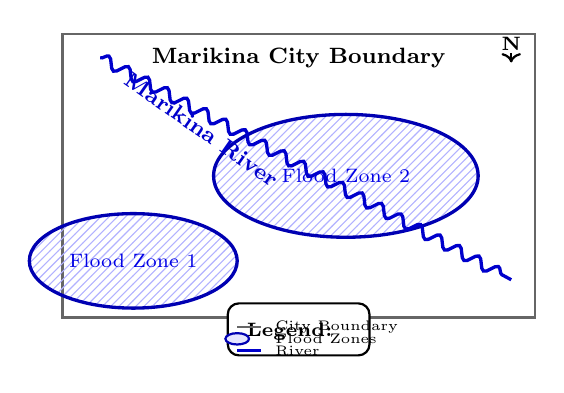
\begin{tikzpicture}[scale=0.6]
    % Map boundary (Marikina City)
    \draw[thick,black!60] (0,0) rectangle (10,6);
    \node[anchor=center,font=\footnotesize\bfseries] at (5,5.5) {Marikina City Boundary};
    
    % Flood zones (blue ellipses with reduced opacity)
    \draw[fill=blue!10,draw=blue!70!black,very thick,pattern=north east lines,pattern color=blue!30] (1.5,1.2) ellipse (2.2 and 1.0);
    \node[anchor=center,font=\scriptsize,text=blue!90!black] at (1.5,1.2) {Flood Zone 1};
    
    \draw[fill=blue!10,draw=blue!70!black,very thick,pattern=north east lines,pattern color=blue!30] (6,3) ellipse (2.8 and 1.3);
    \node[anchor=center,font=\scriptsize,text=blue!90!black] at (6,3) {Flood Zone 2};
    
    % Marikina River (wavy blue line)
    \draw[very thick,blue!80!black,decorate,decoration={snake,amplitude=2pt,segment length=8pt}] (0.8,5.5) -- (9.5,0.8);
    \node[anchor=west,font=\footnotesize\bfseries,text=blue!80!black,rotate=-35] at (1.2,5.2) {Marikina River};
    
    % Reference point (N for North)
    \node[font=\scriptsize\bfseries] at (9.5,5.8) {N};
    \draw[->,thick] (9.5,5.6) -- (9.5,5.4);
    
    % Legend box moved to bottom center
    \draw[fill=white,draw=black,thick,rounded corners] (3.5,-0.8) rectangle (6.5,0.3);
    \node[anchor=north west,font=\scriptsize\bfseries] at (3.7,0.1) {Legend:};
    \draw[thick,black!60] (3.7,-0.2) -- (4.2,-0.2);
    \node[anchor=west,font=\tiny] at (4.3,-0.2) {City Boundary};
    \draw[fill=blue!10,draw=blue!70!black,thick] (3.7,-0.45) ellipse (0.25 and 0.12);
    \node[anchor=west,font=\tiny] at (4.3,-0.45) {Flood Zones};
    \draw[very thick,blue!80!black] (3.7,-0.7) -- (4.2,-0.7);
    \node[anchor=west,font=\tiny] at (4.3,-0.7) {River};
  \end{tikzpicture}}
  \end{center}
  \vspace{2pt}
  \begin{center}\small Traditional navigation failed; residents routed into trap zones\end{center}
\end{frame}

\begin{frame}{Research Gap}
  \footnotesize
  \begin{tabular}{lccccc}
    \toprule
    System & Multi-Agent & Real-Time Flood & Crowdsourced & Risk-Aware & Deployed \\
    \midrule
    MAS-FRO & \(\checkmark\) & \(\checkmark\) & \(\checkmark\) & \(\checkmark\) & Prototype \\
    Google Maps & \(\times\) & \(\times\) & \(\checkmark\) (traffic) & \(\times\) & \(\checkmark\) \\
    DOST-NOAH & \(\times\) & \(\checkmark\) & \(\times\) & \(\times\) (monitor) & \(\checkmark\) \\
    Academic MAS & \(\checkmark\) & \(\times\) & \(\times\) & \(\times\) & \(\times\) (sim) \\
    \bottomrule
  \end{tabular}
  \vspace{6pt}
  \begin{block}{Conclusion}
    No existing system combines all four capabilities in an operational prototype.
  \end{block}
\end{frame}

\begin{frame}{Marikina City Context}
  \vspace{-6pt}
  \begin{center}
  \small Boundary: \SI{21.5}{\kilo\meter\squared}; Population: \(\sim\)450,000 | Road network: \(\abs{V}\approx 10{,}000\), \(\abs{E}\approx 20{,}000\)
  \end{center}
  \vspace{4pt}
  \begin{center}
  \adjustbox{width=0.88\textwidth,center}{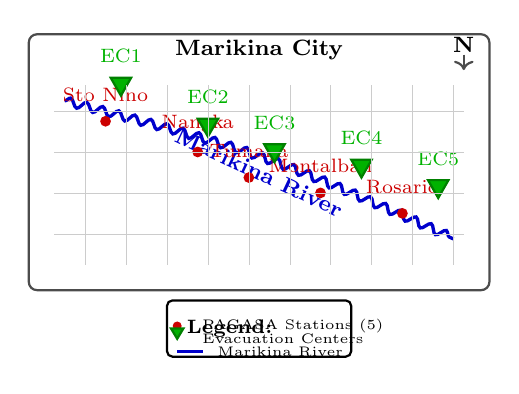
\begin{tikzpicture}[scale=0.65]
    % City boundary
    \draw[thick,black!70,rounded corners=3pt] (0.5,0.5) rectangle (9.5,5.5);
    \node[anchor=center,font=\footnotesize\bfseries] at (5,5.2) {Marikina City};
    
    % Marikina River (curved path with label)
    \draw[very thick,blue!80!black,decorate,decoration={snake,amplitude=1.5pt,segment length=6pt}] (1.2,4.2) .. controls (5,3.2) .. (8.8,1.5);
    \node[anchor=center,font=\footnotesize\bfseries,text=blue!80!black,rotate=-25] at (5,2.8) {Marikina River};
    
    % PAGASA stations (red dots with labels) - increased spacing
    \foreach \x/\y/\name in {2/3.8/Sto Nino,3.8/3.2/Nangka,4.8/2.7/Tumana,6.2/2.4/Montalban,7.8/2.0/Rosario}{
      \fill[red!80!black] (\x,\y) circle (3pt);
      \node[anchor=south,font=\scriptsize,text=red!80!black] at (\x,\y+0.2) {\name};
    }
    
    % Evacuation centers (green triangles) - repositioned to avoid overlap
    \foreach \x/\y/\num in {2.3/4.3/1,4.0/3.5/2,5.3/3.0/3,7.0/2.7/4,8.5/2.3/5}{
      \draw[fill=green!70!black,draw=green!50!black,thick] (\x,\y) -- +(0.2,0.35) -- +(-0.2,0.35) -- cycle;
      \node[anchor=south,font=\scriptsize,text=green!70!black] at (\x,\y+0.45) {EC\num};
    }
    
    % Road network (simplified grid, lighter)
    \draw[gray!40,very thin] (1,1) grid[step=0.8] (9,4.5);
    
    % Compass rose
    \node[font=\footnotesize\bfseries] at (9.0,5.3) {N};
    \draw[->,thick,black!70] (9.0,5.1) -- (9.0,4.8);
    
    % Legend box moved to bottom center
    \draw[fill=white,draw=black,thick,rounded corners=2pt] (3.2,-0.8) rectangle (6.8,0.3);
    \node[anchor=north west,font=\scriptsize\bfseries] at (3.4,0.1) {Legend:};
    \fill[red!80!black] (3.4,-0.2) circle (2.5pt);
    \node[anchor=west,font=\tiny] at (3.7,-0.2) {PAGASA Stations (5)};
    \draw[fill=green!70!black,draw=green!50!black,thick] (3.4,-0.45) -- +(0.12,0.2) -- +(-0.12,0.2) -- cycle;
    \node[anchor=west,font=\tiny] at (3.7,-0.45) {Evacuation Centers};
    \draw[very thick,blue!80!black] (3.4,-0.7) -- (3.9,-0.7);
    \node[anchor=west,font=\tiny] at (4.0,-0.7) {Marikina River};
  \end{tikzpicture}}
  \end{center}
\end{frame}

\begin{frame}{Five Challenges}
  \begin{enumerate}
    \item Dynamic hazards: flood depth changes in minutes
    \item Multi-source data: PAGASA + OpenWeatherMap + GeoTIFF + Twitter/X
    \item Real-time performance: \(<2\)s route computation
    \item Data reliability: official sparse; crowdsourced noisy
    \item 24/7 availability: graceful degradation when APIs fail
  \end{enumerate}
\end{frame}

\begin{frame}{Research Objectives}
  \begin{itemize}
    \item Primary: Real-time flood-safe routing for Marikina City
    \item Specific aims:
    \begin{enumerate}
      \item Design hierarchical MAS (FIPA-ACL)
      \item Integrate real-time data sources (PAGASA, OWM, GeoTIFF)
      \item Implement risk-aware A* pathfinding
      \item Develop web prototype (Next.js + FastAPI)
      \item Validate performance (\alert{pending} comparative evaluation)
    \end{enumerate}
  \end{itemize}
\end{frame}

\begin{frame}{Scope \& Limitations (Upfront Honesty)}
  \small
  \begin{columns}[T,onlytextwidth]
    \column{0.33\textwidth}
      \textbf{In Scope}
      \begin{itemize}\itemsep2pt
        \item Marikina City only
        \item 5+ months operational (projected)
        \item Real APIs integrated
      \end{itemize}
    \column{0.33\textwidth}
      \textbf{Out of Scope}
      \begin{itemize}\itemsep2pt
        \item Other cities
        \item Multi-hazard
        \item Offline mode
      \end{itemize}
    \column{0.33\textwidth}
      \textbf{Validation Gaps}
      \begin{itemize}\itemsep2pt
        \item No baseline
        \item No real emergency deployment
        \item Expert validation pending
      \end{itemize}
  \end{columns}
\end{frame}

% ============================================
% SECTION: Theoretical Foundations
% ============================================
\section{Theoretical Foundations}

% -------------------------
% Theory (4)
% -------------------------
\begin{frame}{Multi-Agent Systems Theory}
  \small
  \begin{itemize}
    \item Wooldridge (1995): autonomy, reactivity, proactivity, social ability
  \end{itemize}
  \vspace{6pt}
  \begin{tabular}{lccc}
    \toprule
    Property & FloodAgent & HazardAgent & RoutingAgent \\
    \midrule
    Autonomy & \(\checkmark\) (5-min) & \(\checkmark\) (fusion) & \(\checkmark\) (on-demand) \\
    Reactivity & \(\checkmark\) & \(\checkmark\) & \(\checkmark\) \\
    Proactivity & \(\checkmark\) & \(\checkmark\) & \(\checkmark\) \\
    Social Ability & \(\checkmark\) (INFORM) & \(\checkmark\) & \(\checkmark\) (REQUEST/CONFIRM) \\
    \bottomrule
  \end{tabular}
  \vspace{6pt}
  \begin{block}{FIPA-ACL}
    Standard performatives for agent communication (REQUEST, INFORM, CONFIRM, \dots)
  \end{block}
\end{frame}

\begin{frame}{Graph Theory \& A* Algorithm}
  \small
  \begin{itemize}
    \item Road network: directed multi-graph \(G=(V,E,W)\), \(\abs{V}\approx 10{,}000\), \(\abs{E}\approx 20{,}000\)
    \item A*: \(f(n)=g(n)+h(n)\). If \(h\) admissible \(\Rightarrow\) optimal path
    \item Haversine heuristic; Complexity: \(\mathcal{O}((\abs{V}+\abs{E})\log \abs{V})\)
  \end{itemize}
  \vspace{6pt}
  \begin{block}{Heuristic}
    Great-circle approximation sufficient at Marikina scale (\(<50\)m error typical).
  \end{block}
\end{frame}

\begin{frame}{Risk Assessment \& MCDM}
  \small
  \begin{itemize}
    \item Weighted sum: \( \text{Cost} = w_d \cdot \text{distance} + w_r \cdot \text{risk} \)
    \item Current weights: \(w_d=0.4\), \(w_r=0.6\) (\emph{heuristic}; to be calibrated)
  \end{itemize}
  \vspace{6pt}
  \begin{block}{Passability Constraint}
    If \(r(e)\ge 0.9\Rightarrow C(e)=\infty\) (edge blocked).
  \end{block}
\end{frame}

\begin{frame}{Data Fusion (Terminology Correction)}
  \small
  \textbf{Simplified Bayesian-Inspired Weighted Aggregation}
  \[
    R_{\text{fused}}=\alpha_1 R_{\text{official}}+\alpha_2 R_{\text{crowd}}+\alpha_3 R_{\text{hist}}
  \]
  \(\alpha_1=0.5, \alpha_2=0.3, \alpha_3=0.2\)
  \begin{block}{Note}
    Weighted averaging, not full Bayesian inference. Future work: full Bayesian model with priors and likelihoods.
  \end{block}
\end{frame}

% ============================================
% SECTION: Related Work
% ============================================
\section{Related Work}

% -------------------------
% Related Work (3)
% -------------------------
\begin{frame}{Related Work - Categories}
  \small
  \begin{enumerate}\itemsep4pt
    \item Disaster routing (offline planning)
    \item Commercial navigation (no flood awareness)
    \item Government monitoring (no routing)
    \item Multi-agent simulation (not deployed)
    \item Philippine systems (monitoring only)
  \end{enumerate}
  \vspace{4pt}
  \alert{Gap:} No paper/system combines MAS + real-time flood + operational prototype.
\end{frame}

\begin{frame}{Risk-Aware Pathfinding Timeline}
  \vspace{-4pt}
  \begin{center}
  \adjustbox{width=0.92\textwidth,center}{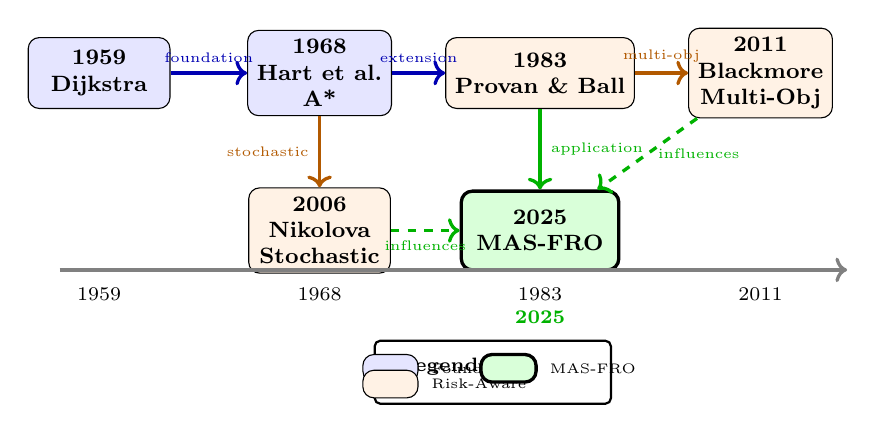
\begin{tikzpicture}[
    milestone/.style={draw,rounded corners,fill=blue!10,minimum width=1.8cm,minimum height=0.9cm,align=center,font=\footnotesize\bfseries},
    risk-aware/.style={draw,rounded corners,fill=orange!10,minimum width=1.8cm,minimum height=0.9cm,align=center,font=\footnotesize\bfseries},
    current/.style={draw,rounded corners,fill=green!15,minimum width=2.0cm,minimum height=1.0cm,align=center,font=\footnotesize\bfseries,very thick}
  ]
    % Timeline nodes with increased vertical spacing
    \node[milestone] (n1) at (0,3) {\textbf{1959}\\Dijkstra};
    \node[milestone] (n2) at (2.8,3) {\textbf{1968}\\Hart et al.\\A*};
    \node[risk-aware] (n3) at (5.6,3) {\textbf{1983}\\Provan \& Ball};
    \node[risk-aware] (n4) at (2.8,1) {\textbf{2006}\\Nikolova\\Stochastic};
    \node[risk-aware] (n5) at (8.4,3) {\textbf{2011}\\Blackmore\\Multi-Obj};
    \node[current] (n6) at (5.6,1) {\textbf{2025}\\MAS-FRO};
    
    % Timeline axis
    \draw[->,very thick,black!50] (-0.5,0.5) -- (9.5,0.5);
    \node[anchor=north,font=\scriptsize] at (0,0.4) {1959};
    \node[anchor=north,font=\scriptsize] at (2.8,0.4) {1968};
    \node[anchor=north,font=\scriptsize] at (5.6,0.4) {1983};
    \node[anchor=north,font=\scriptsize] at (8.4,0.4) {2011};
    \node[anchor=north,font=\scriptsize\bfseries,text=green!70!black] at (5.6,0.1) {2025};
    
    % Simplified connections - removed redundant arrows
    \draw[->,very thick,blue!70!black] (n1) -- node[above,font=\tiny] {foundation} (n2);
    \draw[->,very thick,blue!70!black] (n2) -- node[above,font=\tiny] {extension} (n3);
    \draw[->,very thick,orange!70!black] (n2) -- node[left,font=\tiny] {stochastic} (n4);
    \draw[->,very thick,orange!70!black] (n3) -- node[above,font=\tiny] {multi-obj} (n5);
    \draw[->,very thick,green!70!black] (n3) -- node[right,font=\tiny] {application} (n6);
    \draw[->,very thick,green!70!black,dashed] (n4) -- node[below,font=\tiny] {influences} (n6);
    \draw[->,very thick,green!70!black,dashed] (n5) -- node[right,font=\tiny] {influences} (n6);
    
    % Legend moved to bottom
    \draw[fill=white,draw=black,thick,rounded corners=2pt] (3.5,-1.2) rectangle (6.5,-0.4);
    \node[anchor=north west,font=\scriptsize\bfseries] at (3.7,-0.5) {Legend:};
    \node[milestone,minimum width=0.7cm,minimum height=0.35cm,font=\tiny] at (3.7,-0.75) {};
    \node[anchor=west,font=\tiny] at (4.1,-0.75) {Foundation};
    \node[risk-aware,minimum width=0.7cm,minimum height=0.35cm,font=\tiny] at (3.7,-0.95) {};
    \node[anchor=west,font=\tiny] at (4.1,-0.95) {Risk-Aware};
    \node[current,minimum width=0.7cm,minimum height=0.35cm,font=\tiny] at (5.2,-0.75) {};
    \node[anchor=west,font=\tiny] at (5.6,-0.75) {MAS-FRO};
  \end{tikzpicture}}
  \end{center}
  \vspace{4pt}
  \begin{center}\small Application of established techniques to a novel operational domain (flood evacuation).\end{center}
\end{frame}

\begin{frame}{MAS-FRO Unique Niche}
  \vspace{-4pt}
  \begin{center}
  \adjustbox{width=0.85\textwidth,center}{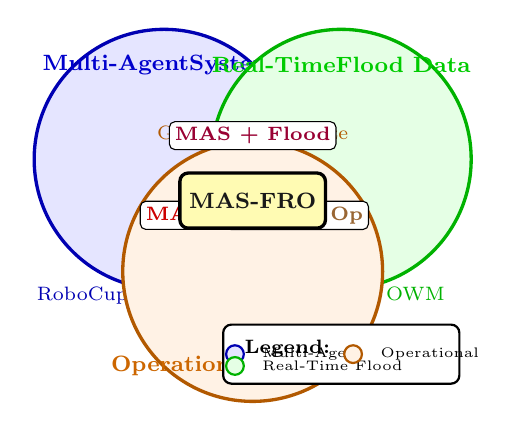
\begin{tikzpicture}[scale=0.75]
    \def\r{2.2}
    % Circle 1: Multi-Agent - increased separation
    \begin{scope}[shift={(0,0)}]
      \draw[fill=blue!10,draw=blue!70!black,very thick] (0,0) circle (\r);
      \node[font=\footnotesize\bfseries,text=blue!80!black] at (0,1.6) {Multi-Agent\\Systems};
      \node[font=\scriptsize,text=blue!70!black,anchor=north] at (0,-2.0) {RoboCup, Academic MAS};
    \end{scope}
    % Circle 2: Real-Time Flood - increased separation
    \begin{scope}[shift={(3.0,0)}]
      \draw[fill=green!10,draw=green!70!black,very thick] (0,0) circle (\r);
      \node[font=\footnotesize\bfseries,text=green!80!black] at (0,1.6) {Real-Time\\Flood Data};
      \node[font=\scriptsize,text=green!70!black,anchor=north] at (0,-2.0) {DOST-NOAH, OWM};
    \end{scope}
    % Circle 3: Operational - repositioned
    \begin{scope}[shift={(1.5,-1.9)}]
      \draw[fill=orange!10,draw=orange!70!black,very thick] (0,0) circle (\r);
      \node[font=\footnotesize\bfseries,text=orange!80!black] at (0,-1.6) {Operational\\Deployment};
      \node[font=\scriptsize,text=orange!70!black,anchor=south] at (0,2.0) {Google Maps, Waze};
    \end{scope}
    
    % Intersection labels - better positioned with white background
    \node[draw,fill=white,rounded corners=2pt,font=\scriptsize\bfseries,text=purple!80!black,inner sep=2pt] at (1.5,0.4) {MAS + Flood};
    \node[draw,fill=white,rounded corners=2pt,font=\scriptsize\bfseries,text=red!80!black,inner sep=2pt] at (0.75,-0.95) {MAS + Op};
    \node[draw,fill=white,rounded corners=2pt,font=\scriptsize\bfseries,text=brown!80!black,inner sep=2pt] at (2.25,-0.95) {Flood + Op};
    
    % Center intersection (MAS-FRO) - larger with better contrast
    \node[draw,very thick,fill=yellow!30,rounded corners=3pt,font=\footnotesize\bfseries,minimum width=1.6cm,minimum height=0.7cm,text=black!90] at (1.5,-0.7) {MAS-FRO};
    
    % Legend moved to bottom
    \draw[fill=white,draw=black,thick,rounded corners=3pt] (1.0,-3.8) rectangle (5.0,-2.8);
    \node[anchor=north west,font=\scriptsize\bfseries] at (1.2,-2.9) {Legend:};
    \draw[fill=blue!10,draw=blue!70!black,thick] (1.2,-3.3) circle (0.15);
    \node[anchor=west,font=\tiny] at (1.5,-3.3) {Multi-Agent};
    \draw[fill=green!10,draw=green!70!black,thick] (1.2,-3.5) circle (0.15);
    \node[anchor=west,font=\tiny] at (1.5,-3.5) {Real-Time Flood};
    \draw[fill=orange!10,draw=orange!70!black,thick] (3.2,-3.3) circle (0.15);
    \node[anchor=west,font=\tiny] at (3.5,-3.3) {Operational};
  \end{tikzpicture}}
  \end{center}
  \vspace{4pt}
  \begin{center}\small \textbf{Unique Position:} Only MAS-FRO combines all three capabilities in an operational prototype.\end{center}
\end{frame}

% ============================================
% SECTION: System Architecture
% ============================================
\section{System Architecture}

% -------------------------
% System Architecture (10)
% -------------------------
\begin{frame}{Architecture Overview}
  \vspace{-4pt}
  \begin{center}
  \adjustbox{width=0.9\textwidth,center}{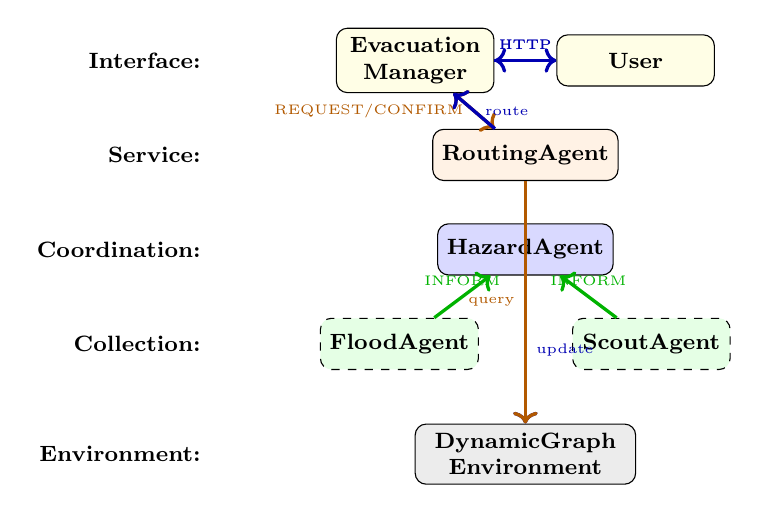
\begin{tikzpicture}[
    interface/.style={draw,rounded corners,fill=yellow!10,minimum width=2.0cm,minimum height=0.65cm,align=center,font=\footnotesize\bfseries},
    service/.style={draw,rounded corners,fill=orange!10,minimum width=2.0cm,minimum height=0.65cm,align=center,font=\footnotesize\bfseries},
    coordinator/.style={draw,rounded corners,fill=blue!15,minimum width=2.0cm,minimum height=0.65cm,align=center,font=\footnotesize\bfseries},
    collector/.style={draw,dashed,rounded corners,fill=green!10,minimum width=2.0cm,minimum height=0.65cm,align=center,font=\footnotesize\bfseries},
    env/.style={draw,rounded corners,fill=gray!15,minimum width=2.8cm,minimum height=0.75cm,align=center,font=\footnotesize\bfseries}
  ]
    % Layer labels (on the left) - increased spacing
    \node[anchor=east,font=\footnotesize\bfseries] at (-0.4,6.0) {Interface:};
    \node[anchor=east,font=\footnotesize\bfseries] at (-0.4,4.8) {Service:};
    \node[anchor=east,font=\footnotesize\bfseries] at (-0.4,3.6) {Coordination:};
    \node[anchor=east,font=\footnotesize\bfseries] at (-0.4,2.4) {Collection:};
    \node[anchor=east,font=\footnotesize\bfseries] at (-0.4,1.0) {Environment:};
    
    % Layer 1: Interface Layer
    \node[interface] (evac) at (2.2,6.0) {Evacuation\\Manager};
    \node[interface] (user) at (5.0,6.0) {User};
    
    % Layer 2: Service Layer
    \node[service] (route) at (3.6,4.8) {RoutingAgent};
    
    % Layer 3: Coordination Layer
    \node[coordinator] (haz) at (3.6,3.6) {HazardAgent};
    
    % Layer 4: Data Collection Layer
    \node[collector] (flood) at (2.0,2.4) {FloodAgent};
    \node[collector] (scout) at (5.2,2.4) {ScoutAgent};
    
    % Layer 5: Environment
    \node[env] (env) at (3.6,1.0) {DynamicGraph\\Environment};
    
    % Connections with simplified labels
    \draw[->,very thick,blue!70!black] (user) -- node[above,font=\tiny] {HTTP} (evac);
    \draw[<->,very thick,orange!70!black] (evac) -- node[left,font=\tiny] {REQUEST/\\CONFIRM} (route);
    \draw[->,very thick,green!70!black] (flood) -- node[above,font=\tiny] {INFORM} (haz);
    \draw[->,very thick,green!70!black] (scout) -- node[above,font=\tiny] {INFORM} (haz);
    \draw[->,very thick,blue!70!black] (haz) -- node[right,font=\tiny] {update} (env);
    \draw[->,very thick,orange!70!black] (route) -- node[left,font=\tiny] {query} (env);
    \draw[->,very thick,blue!70!black] (route) -- node[right,font=\tiny] {route} (evac);
    \draw[->,very thick,blue!70!black] (evac) -- node[above,font=\tiny] {HTTP} (user);
  \end{tikzpicture}}
  \end{center}
\end{frame}

\begin{frame}{Agent Roles Matrix}
  \footnotesize
  \begin{tabular}{llllll}
    \toprule
    Agent & Type & Role & LOC & File & Status \\
    \midrule
    FloodAgent & Collector & Official data (PAGASA, OWM) & 960 & \texttt{flood\_agent.py} & Operational \\
    ScoutAgent & Collector & Crowdsourced (Twitter/X NLP) & 486 & \texttt{scout\_agent.py} & Operational \\
    HazardAgent & Coordinator & Fusion, risk calculation & 594 & \texttt{hazard\_agent.py} & Operational \\
    RoutingAgent & Service & Risk-aware A* & 459 & \texttt{routing\_agent.py} & Operational \\
    EvacuationMgr & Interface & Requests, feedback & 430 & \texttt{evac\_mgr\_agent.py} & Operational \\
    \bottomrule
  \end{tabular}
\end{frame}

\begin{frame}[fragile]{FIPA-ACL Message Example}
\begin{lstlisting}
ACLMessage(
    performative=Performative.INFORM,
    sender="flood_agent_001",
    receiver="hazard_agent_001",
    content={
        "info_type": "flood_data_update",
        "data": {
            "Sto Nino": {
                "water_level": 15.2,
                "risk_level": "ALERT"
            }
        }
    },
    conversation_id="collection_12345"
)
\end{lstlisting}
\end{frame}

\begin{frame}{Communication Sequence}
  \vspace{-4pt}
  \begin{center}
  \adjustbox{width=0.88\textwidth,center}{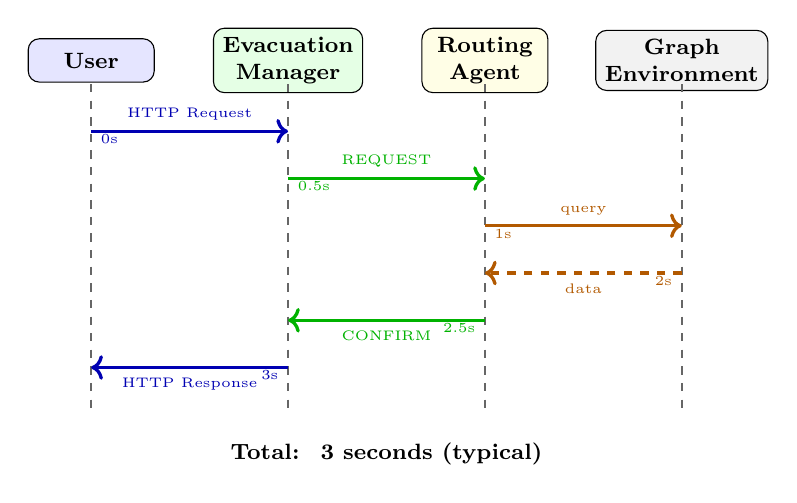
\begin{tikzpicture}[
    lifeline/.style={thick,black!60},
    actor/.style={draw,rounded corners,fill=blue!10,minimum width=1.6cm,minimum height=0.55cm,align=center,font=\footnotesize\bfseries},
    agent/.style={draw,rounded corners,fill=green!10,minimum width=1.6cm,minimum height=0.55cm,align=center,font=\footnotesize\bfseries},
    service/.style={draw,rounded corners,fill=yellow!10,minimum width=1.6cm,minimum height=0.55cm,align=center,font=\footnotesize\bfseries},
    env/.style={draw,rounded corners,fill=gray!10,minimum width=1.6cm,minimum height=0.55cm,align=center,font=\footnotesize\bfseries}
  ]
    % Actors/Agents at top - reduced vertical extent
    \node[actor] (user) at (1,5.5) {User};
    \node[agent] (evac) at (3.5,5.5) {Evacuation\\Manager};
    \node[service] (route) at (6,5.5) {Routing\\Agent};
    \node[env] (graph) at (8.5,5.5) {Graph\\Environment};
    
    % Lifelines (vertical dashed lines) - shortened
    \draw[lifeline,dashed] (1,5.2) -- (1,1);
    \draw[lifeline,dashed] (3.5,5.2) -- (3.5,1);
    \draw[lifeline,dashed] (6,5.2) -- (6,1);
    \draw[lifeline,dashed] (8.5,5.2) -- (8.5,1);
    
    % Messages (horizontal arrows with timing) - condensed spacing
    % T=0s: User -> EvacMgr
    \draw[->,very thick,blue!70!black] (1,4.6) -- node[above,font=\tiny] {HTTP Request} (3.5,4.6);
    \node[anchor=west,font=\tiny,text=blue!70!black] at (1,4.5) {0s};
    
    % T=0.5s: EvacMgr -> RoutingAgent
    \draw[->,very thick,green!70!black] (3.5,4.0) -- node[above,font=\tiny] {REQUEST} (6,4.0);
    \node[anchor=west,font=\tiny,text=green!70!black] at (3.5,3.9) {0.5s};
    
    % T=1s: RoutingAgent -> Graph
    \draw[->,very thick,orange!70!black] (6,3.4) -- node[above,font=\tiny] {query} (8.5,3.4);
    \node[anchor=west,font=\tiny,text=orange!70!black] at (6,3.3) {1s};
    
    % T=2s: Graph -> RoutingAgent (response)
    \draw[->,very thick,orange!70!black,dashed] (8.5,2.8) -- node[below,font=\tiny] {data} (6,2.8);
    \node[anchor=east,font=\tiny,text=orange!70!black] at (8.5,2.7) {2s};
    
    % T=2.5s: RoutingAgent -> EvacMgr
    \draw[->,very thick,green!70!black] (6,2.2) -- node[below,font=\tiny] {CONFIRM} (3.5,2.2);
    \node[anchor=east,font=\tiny,text=green!70!black] at (6,2.1) {2.5s};
    
    % T=3s: EvacMgr -> User
    \draw[->,very thick,blue!70!black] (3.5,1.6) -- node[below,font=\tiny] {HTTP Response} (1,1.6);
    \node[anchor=east,font=\tiny,text=blue!70!black] at (3.5,1.5) {3s};
    
    % Timeline label at bottom
    \node[anchor=center,font=\footnotesize\bfseries] at (4.75,0.5) {Total: ~3 seconds (typical)};
  \end{tikzpicture}}
  \end{center}
\end{frame}

\begin{frame}{Dynamic Graph Environment}
  \vspace{-6pt}
  \begin{center}
  \small Edge weights: \(W(e,t)= \text{length}(e)\cdot r(e,t)\) | Risk: green (low) \(\rightarrow\) orange (medium) \(\rightarrow\) red (high) | Update: 5 minutes
  \end{center}
  \vspace{6pt}
  \begin{center}
  \adjustbox{width=0.88\textwidth,center}{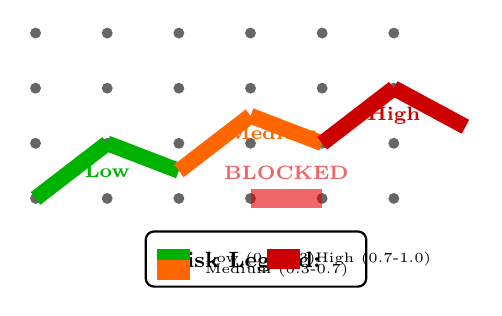
\begin{tikzpicture}[scale=0.7]
    % Road network nodes (intersections)
    \foreach \i in {0,...,5}{
      \foreach \j in {0,...,3}{
        \filldraw[black!60] (1+1.3*\i,0.8+1.0*\j) circle (2.5pt);
      }
    }
    
    % Low risk edges (green) - simplified labels
    \draw[line width=2mm,green!70!black] (1,0.8) -- (2.3,1.8);
    \draw[line width=2mm,green!70!black] (2.3,1.8) -- (3.6,1.3);
    \node[anchor=center,font=\scriptsize\bfseries,text=green!70!black] at (2.3,1.3) {Low};
    
    % Medium risk edges (orange)
    \draw[line width=2mm,orange!80!red] (3.6,1.3) -- (4.9,2.3);
    \draw[line width=2mm,orange!80!red] (4.9,2.3) -- (6.2,1.8);
    \node[anchor=center,font=\scriptsize\bfseries,text=orange!80!red] at (5.3,2.0) {Medium};
    
    % High risk edges (red)
    \draw[line width=2mm,red!80!black] (6.2,1.8) -- (7.5,2.8);
    \draw[line width=2mm,red!80!black] (7.5,2.8) -- (8.8,2.1);
    \node[anchor=center,font=\scriptsize\bfseries,text=red!80!black] at (7.5,2.3) {High};
    
    % Blocked edge (very high risk)
    \draw[line width=2.5mm,red!90!black,opacity=0.6] (4.9,0.8) -- node[above,sloped,font=\scriptsize\bfseries,text=red!90!black] {BLOCKED} (6.2,0.8);
    
    % Legend box moved to bottom
    \draw[fill=white,draw=black,thick,rounded corners=3pt] (3.0,-0.8) rectangle (7.0,0.2);
    \node[anchor=north west,font=\footnotesize\bfseries] at (3.2,0.0) {Risk Legend:};
    \draw[line width=2.5mm,green!70!black] (3.2,-0.3) -- (3.8,-0.3);
    \node[anchor=west,font=\tiny] at (3.9,-0.3) {Low (0.0-0.3)};
    \draw[line width=2.5mm,orange!80!red] (3.2,-0.5) -- (3.8,-0.5);
    \node[anchor=west,font=\tiny] at (3.9,-0.5) {Medium (0.3-0.7)};
    \draw[line width=2.5mm,red!80!black] (5.2,-0.3) -- (5.8,-0.3);
    \node[anchor=west,font=\tiny] at (5.9,-0.3) {High (0.7-1.0)};
  \end{tikzpicture}}
  \end{center}
\end{frame}

\begin{frame}[fragile]{Risk-Aware A*: Balancing Safety and Distance}
  \begin{columns}[T,onlytextwidth]
    \column{0.52\textwidth}
      \small
      \( C(e) =
      \begin{cases}
        \infty & r(e)\ge 0.9 \\
        w_d \cdot d(e) + w_r \cdot d(e)\cdot r(e) & \text{otherwise}
      \end{cases}\)
      \vspace{8pt}

      \(\Rightarrow\) \(\text{Cost}(P)=\sum_{e\in P} C(e)\), minimize over all paths
    \column{0.46\textwidth}
\begin{lstlisting}
def weight_function(u, v, edge_data):
    length = edge_data['length']
    risk = edge_data['risk_score']
    if risk >= 0.9:
        return float('inf')
    return w_d * length + w_r * length * risk
\end{lstlisting}
  \end{columns}
\end{frame}

\begin{frame}{Multi-Source Data Fusion}
  \vspace{-4pt}
  \begin{center}
  \adjustbox{width=0.88\textwidth,center}{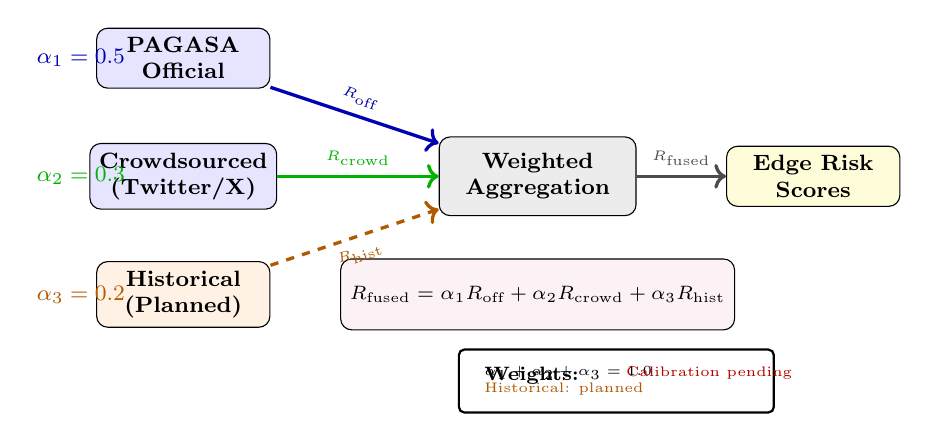
\begin{tikzpicture}[
    source/.style={draw,rounded corners,fill=blue!10,minimum width=2.2cm,minimum height=0.7cm,align=center,font=\footnotesize\bfseries},
    process/.style={draw,rounded corners,fill=gray!15,minimum width=2.5cm,minimum height=1.0cm,align=center,font=\footnotesize\bfseries},
    output/.style={draw,rounded corners,fill=yellow!15,minimum width=2.2cm,minimum height=0.7cm,align=center,font=\footnotesize\bfseries},
    formula/.style={draw,rounded corners,fill=purple!5,minimum width=3.5cm,minimum height=0.9cm,align=center,font=\scriptsize}
  ]
    % Data sources - increased vertical spacing
    \node[source] (p1) at (0,3.5) {PAGASA\\Official};
    \node[source] (p2) at (0,2.0) {Crowdsourced\\(Twitter/X)};
    \node[source,fill=orange!10] (p3) at (0,0.5) {Historical\\(Planned)};
    
    % Weight labels - repositioned to avoid overlap
    \node[font=\footnotesize\bfseries,text=blue!70!black] at (-1.3,3.5) {\(\alpha_1=0.5\)};
    \node[font=\footnotesize\bfseries,text=green!70!black] at (-1.3,2.0) {\(\alpha_2=0.3\)};
    \node[font=\footnotesize\bfseries,text=orange!70!black] at (-1.3,0.5) {\(\alpha_3=0.2\)};
    
    % Fusion process with formula
    \node[process] (fuse) at (4.5,2.0) {Weighted\\Aggregation};
    \node[formula] at (4.5,0.5) {\(R_{\text{fused}} = \alpha_1 R_{\text{off}} + \alpha_2 R_{\text{crowd}} + \alpha_3 R_{\text{hist}}\)};
    
    % Output
    \node[output] (out) at (8,2.0) {Edge Risk\\Scores};
    
    % Arrows with labels
    \draw[->,very thick,blue!70!black] (p1) -- node[above,font=\tiny,sloped] {\(R_{\text{off}}\)} (fuse);
    \draw[->,very thick,green!70!black] (p2) -- node[above,font=\tiny,sloped] {\(R_{\text{crowd}}\)} (fuse);
    \draw[->,very thick,orange!70!black,dashed] (p3) -- node[below,font=\tiny,sloped] {\(R_{\text{hist}}\)} (fuse);
    \draw[->,very thick,black!70] (fuse) -- node[above,font=\tiny] {\(R_{\text{fused}}\)} (out);
    
    % Weight explanation moved to bottom
    \draw[fill=white,draw=black,thick,rounded corners=2pt] (3.5,-1.0) rectangle (7.5,-0.2);
    \node[anchor=north west,font=\scriptsize\bfseries] at (3.7,-0.3) {Weights:};
    \node[anchor=west,font=\tiny] at (3.7,-0.5) {\(\alpha_1 + \alpha_2 + \alpha_3 = 1.0\)};
    \node[anchor=west,font=\tiny,text=orange!70!black] at (3.7,-0.7) {Historical: planned};
    \node[anchor=west,font=\tiny,text=red!70!black] at (5.5,-0.5) {Calibration pending};
  \end{tikzpicture}}
  \end{center}
  \vspace{4pt}
  \begin{center}\small \alert{Weights heuristic; empirical calibration pending (publication gap).}\end{center}
\end{frame}

\begin{frame}[fragile]{FloodAgent Implementation (Key Method)}
\begin{lstlisting}
def fetch_real_river_levels(self) -> Dict:
    """Fetch from PAGASA API, filter Marikina stations."""
    stations = self.river_scraper.get_river_levels()  # 17 stations
    marikina_stations = ["Sto Nino", "Nangka", "Tumana",
                         "Montalban", "Rosario Bridge"]
    filtered = {s['name']: classify_risk(s['water_level'],
                                         s['critical_level'])
                for s in stations if s['name'] in marikina_stations}
    return filtered  # 5 stations
\end{lstlisting}
\end{frame}

\begin{frame}[fragile]{HazardAgent Implementation (Fusion Logic)}
\begin{lstlisting}
def fuse_data(self) -> Dict[str, Any]:
    """Weighted multi-source aggregation."""
    fused = {}
    for edge in graph.edges():
        depth = geotiff.get_depth(edge_midpoint)  # official
        R_official = map_depth_to_risk(depth)
        reports = find_reports_within_500m(edge)  # crowd
        R_crowd = average_severity(reports)
        risk = 0.5*R_official + 0.3*R_crowd + 0.2*R_hist
        fused[edge] = min(risk, 1.0)
    return fused
\end{lstlisting}
\end{frame}

\begin{frame}{System Statistics}
  \begin{itemize}
    \item 5 Autonomous Agents; \(\sim\)8,000 LOC
    \item PAGASA stations: 17\(\rightarrow\)5 (Marikina-filtered)
    \item 72 GeoTIFF flood maps; \(\abs{V}\approx 10{,}000\), \(\abs{E}\approx 20{,}000\)
    \item Update cycle: \SI{5}{\minute}; 95\% real data
  \end{itemize}
\end{frame}

% ============================================
% SECTION: Agreement Form Compliance
% ============================================
\section{Agreement Form Compliance}

% -------------------------
% Agreement Form Compliance (8)
% -------------------------
\begin{frame}{Agreement Form Overview}
  \small
  \begin{tabular}{llll}
    \toprule
    Item & Description & Status & Gap \\
    \midrule
    1 & MAS Communication & \statuspartial{4/5} & Stress testing \\
    2 & Dynamic Graph & \statuscomplete{5/5} & Calibration pending \\
    3 & Baseline & \statusmissing{0/3} & \textbf{CRITICAL} \\
    4 & Risk-Aware A* & \statuscomplete{Complete} & -- \\
    5 & Simulation & \statuspartial{2/4} & Systematic testing \\
    6 & Web Prototype & \statuscomplete{Complete} & -- \\
    7 & Paper & \statusmissing{Rejected} & 3,5,1.v \\
    \bottomrule
  \end{tabular}
\end{frame}

\begin{frame}{Item 1 - MAS Communication (4/5)}
  \small
  \begin{itemize}
    \item \(\checkmark\) Roles defined (5 agents)
    \item \(\checkmark\) Middleware (FIPA-ACL)
    \item \(\checkmark\) Message formats (dataclass, 9 performatives)
    \item \(\triangle\) Failover: graceful degradation only
    \item \(\times\) Network stress testing (not conducted)
  \end{itemize}
  Evidence: \texttt{app/communication/acl\_protocol.py}, \texttt{message\_queue.py}
\end{frame}

\begin{frame}{Item 2 - Dynamic Graph (5/5)}
  \small
  \begin{itemize}
    \item \(\checkmark\) NetworkX MultiDiGraph; OSMnx (Marikina)
    \item \(\checkmark\) 72 GeoTIFF hazard maps
    \item \(\checkmark\) Real-time updates (5-min cadence)
    \item \(\checkmark\) Hazard scoring implemented (\emph{weights heuristic})
  \end{itemize}
  Caveat: Weight calibration pending.
\end{frame}

\begin{frame}{Item 3 - Baseline (\statusmissing{Critical Gap})}
  \small
  \begin{itemize}
    \item 0/3 complete: centralized baseline, time/accuracy/scalability comparisons absent
    \item Primary reason for paper rejection
    \item Roadmap: 16–20 hours to implement \& test
  \end{itemize}
\end{frame}

\begin{frame}{Item 4 - Risk-Aware A* (Complete)}
  \small
  \[
    P^*=\argmin_{P\in\mathcal{P}(s,t)} \sum_{e\in P} C(e),\quad
    C(e)=
    \begin{cases}
      \infty & r(e)\ge 0.9\\
      w_d d(e)+ w_r d(e) r(e) & \text{otherwise}
    \end{cases}
  \]
  Complexity: \(\mathcal{O}((\abs{V}+\abs{E})\log \abs{V})\).
\end{frame}

\begin{frame}{Item 5 - Simulation Testing (2/4)}
  \small
  \begin{itemize}
    \item \(\checkmark\) Agent instances configured
    \item \(\triangle\) Multi-scenario tests exist but not systematic
    \item \(\times\) Metrics collection (manual, \(n\approx 20\))
    \item \(\triangle\) Logs: stdout only
  \end{itemize}
  Gap: Framework + automation (20–24 hours).
\end{frame}

\begin{frame}{Item 6 - Web Prototype (Complete)}
  \small
  \begin{itemize}
    \item Next.js 15 + Mapbox GL; 18+ REST endpoints
    \item WebSocket (5-min updates); PostgreSQL (5+ months data, projected)
    \item Status: Functional prototype (\emph{not} production-hardened)
  \end{itemize}
\end{frame}

\begin{frame}{Item 7 - Paper Status (Rejected)}
  \small
  Probable reasons:
  \begin{enumerate}
    \item No baseline comparison
    \item No systematic validation
    \item No stress testing
    \item Incomplete calibration
    \item Overstated novelty
  \end{enumerate}
  \vspace{4pt}
  Roadmap: Phase 1 (56–72h) to close 3,5,1.v; Phase 2: real-world validation.
\end{frame}

% ============================================
% SECTION: Implementation Highlights
% ============================================
\section{Implementation Highlights}

% -------------------------
% Implementation Highlights (5)
% -------------------------
\begin{frame}{Real-Time Data Integration}
  \vspace{-4pt}
  \begin{center}
  \adjustbox{width=0.88\textwidth,center}{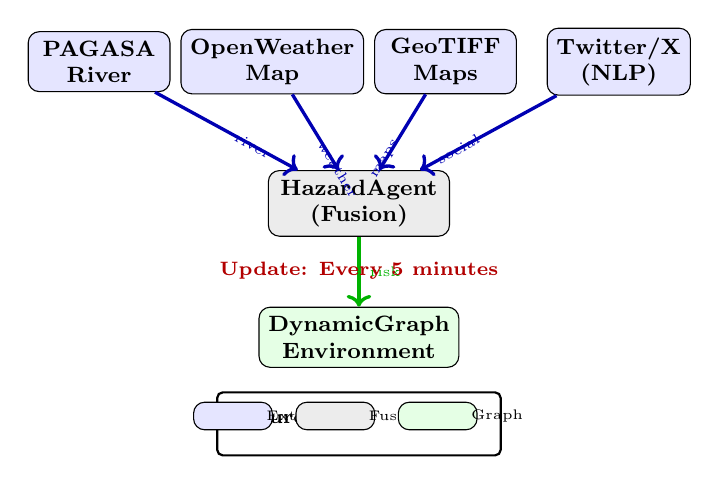
\begin{tikzpicture}[
    source/.style={draw,rounded corners,fill=blue!10,minimum width=1.8cm,minimum height=0.65cm,align=center,font=\footnotesize\bfseries},
    agent/.style={draw,rounded corners,fill=gray!15,minimum width=2.3cm,minimum height=0.75cm,align=center,font=\footnotesize\bfseries},
    env/.style={draw,rounded corners,fill=green!10,minimum width=2.3cm,minimum height=0.75cm,align=center,font=\footnotesize\bfseries}
  ]
    % Data sources - increased horizontal spacing
    \node[source] (p1) at (0,4) {PAGASA\\River};
    \node[source] (p2) at (2.2,4) {OpenWeather\\Map};
    \node[source] (p3) at (4.4,4) {GeoTIFF\\Maps};
    \node[source] (p4) at (6.6,4) {Twitter/X\\(NLP)};
    
    % Source labels - removed to reduce clutter
    % HazardAgent (fusion center)
    \node[agent] (haz) at (3.3,2.2) {HazardAgent\\(Fusion)};
    
    % Graph environment
    \node[env] (graph) at (3.3,0.5) {DynamicGraph\\Environment};
    
    % Arrows with labels - simplified
    \draw[->,very thick,blue!70!black] (p1) -- node[right,font=\tiny,sloped] {river} (haz);
    \draw[->,very thick,blue!70!black] (p2) -- node[right,font=\tiny,sloped] {weather} (haz);
    \draw[->,very thick,blue!70!black] (p3) -- node[left,font=\tiny,sloped] {maps} (haz);
    \draw[->,very thick,blue!70!black] (p4) -- node[left,font=\tiny,sloped] {social} (haz);
    \draw[->,very thick,green!70!black] (haz) -- node[right,font=\tiny] {risk} (graph);
    
    % Update cadence label
    \node[font=\scriptsize\bfseries,text=red!70!black,anchor=center] at (3.3,1.35) {Update: Every 5 minutes};
    
    % Legend moved to bottom - simplified
    \draw[fill=white,draw=black,thick,rounded corners=2pt] (1.5,-1.0) rectangle (5.1,-0.2);
    \node[anchor=north west,font=\scriptsize\bfseries] at (1.7,-0.3) {Sources:};
    \node[source,minimum width=1.0cm,minimum height=0.35cm,font=\tiny] at (1.7,-0.5) {};
    \node[anchor=west,font=\tiny] at (2.0,-0.5) {External API};
    \node[agent,minimum width=1.0cm,minimum height=0.35cm,font=\tiny] at (3.0,-0.5) {};
    \node[anchor=west,font=\tiny] at (3.3,-0.5) {Fusion};
    \node[env,minimum width=1.0cm,minimum height=0.35cm,font=\tiny] at (4.3,-0.5) {};
    \node[anchor=west,font=\tiny] at (4.6,-0.5) {Graph};
  \end{tikzpicture}}
  \end{center}
  \vspace{4pt}
  \begin{center}\small API costs: within free tier. 95\% real data, 5\% simulated fallback.\end{center}
\end{frame}

\begin{frame}{GeoTIFF Service Architecture}
  \small
  \begin{enumerate}\itemsep2pt
    \item Select return period/time-step
    \item Lazy load \texttt{.tif}
    \item LRU cache (max 32)
    \item WGS84 \(\rightarrow\) Web Mercator
    \item Pixel lookup (e.g., 368\(\times\)372 raster)
    \item Return flood depth (m)
  \end{enumerate}
  \vspace{4pt}
  Performance: \(<0.1\)s/query with cache.
\end{frame}

\begin{frame}{WebSocket Real-Time Architecture}
  \vspace{-4pt}
  \begin{center}
  \adjustbox{width=0.88\textwidth,center}{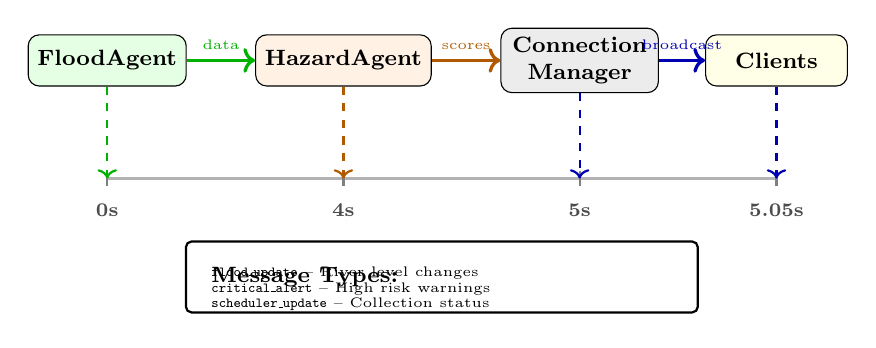
\begin{tikzpicture}[
    agent/.style={draw,rounded corners,fill=green!10,minimum width=1.8cm,minimum height=0.65cm,align=center,font=\footnotesize\bfseries},
    process/.style={draw,rounded corners,fill=orange!10,minimum width=1.8cm,minimum height=0.65cm,align=center,font=\footnotesize\bfseries},
    manager/.style={draw,rounded corners,fill=gray!15,minimum width=2.0cm,minimum height=0.65cm,align=center,font=\footnotesize\bfseries},
    client/.style={draw,rounded corners,fill=yellow!10,minimum width=1.8cm,minimum height=0.65cm,align=center,font=\footnotesize\bfseries}
  ]
    % Components - reduced vertical spacing
    \node[agent] (fa) at (0,3.5) {FloodAgent};
    \node[process] (ha) at (3,3.5) {HazardAgent};
    \node[manager] (cm) at (6,3.5) {Connection\\Manager};
    \node[client] (cli) at (8.5,3.5) {Clients};
    
    % Timeline bar - simplified
    \draw[very thick,black!30] (0,2.0) -- (8.5,2.0);
    \foreach \x/\t in {0/0s,3/4s,6/5s,8.5/5.05s} {
      \draw[thick,black!50] (\x,1.9) -- (\x,2.1);
      \node[anchor=north,font=\scriptsize\bfseries,text=black!70] at (\x,1.8) {\t};
    }
    
    % Data flow arrows - simplified
    \draw[->,very thick,green!70!black] (fa) -- node[above,font=\tiny] {data} (ha);
    \draw[->,very thick,orange!70!black] (ha) -- node[above,font=\tiny] {scores} (cm);
    \draw[->,very thick,blue!70!black] (cm) -- node[above,font=\tiny] {broadcast} (cli);
    
    % Vertical lines to timeline - simplified
    \draw[->,dashed,thick,green!70!black] (fa) -- (0,2.0);
    \draw[->,dashed,thick,orange!70!black] (ha) -- (3,2.0);
    \draw[->,dashed,thick,blue!70!black] (cm) -- (6,2.0);
    \draw[->,dashed,thick,blue!70!black] (cli) -- (8.5,2.0);
    
    % Message types box moved to bottom - simplified
    \draw[fill=white,draw=black,thick,rounded corners=2pt] (1.0,0.3) rectangle (7.5,1.2);
    \node[anchor=north west,font=\footnotesize\bfseries] at (1.2,1.0) {Message Types:};
    \node[anchor=west,font=\tiny] at (1.2,0.8) {\texttt{flood\_update} -- River level changes};
    \node[anchor=west,font=\tiny] at (1.2,0.6) {\texttt{critical\_alert} -- High risk warnings};
    \node[anchor=west,font=\tiny] at (1.2,0.4) {\texttt{scheduler\_update} -- Collection status};
  \end{tikzpicture}}
  \end{center}
  \vspace{4pt}
  \begin{center}\small Total latency: ~5 seconds from data fetch to client update.\end{center}
\end{frame}

\begin{frame}{Database Schema (ER Diagram)}
  \vspace{-4pt}
  \begin{center}
  \adjustbox{width=0.85\textwidth,center}{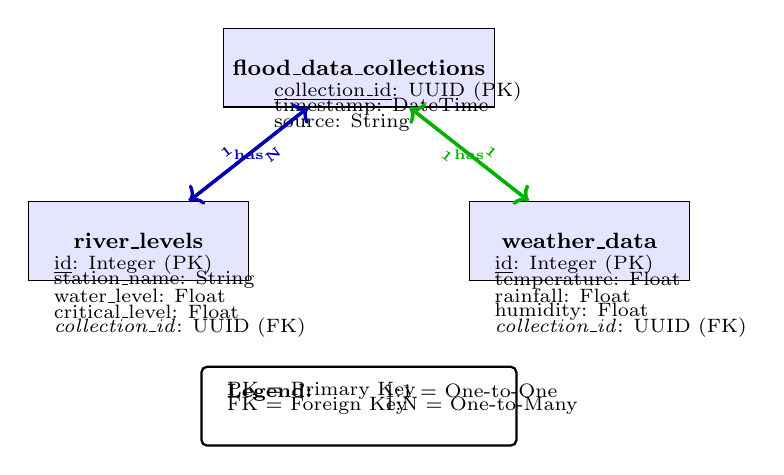
\begin{tikzpicture}[
    entity/.style={draw,rectangle,fill=blue!10,minimum width=2.8cm,minimum height=1.0cm,align=center,font=\footnotesize},
    attr/.style={font=\scriptsize,anchor=west}
  ]
    % Entity: flood_data_collections - increased spacing
    \node[entity] (c) at (0,3.0) {\textbf{flood\_data\_collections}};
    \node[attr] at (-1.2,2.7) {\underline{collection\_id}: UUID (PK)};
    \node[attr] at (-1.2,2.5) {timestamp: DateTime};
    \node[attr] at (-1.2,2.3) {source: String};
    
    % Entity: river_levels - increased spacing
    \node[entity] (r) at (-2.8,0.8) {\textbf{river\_levels}};
    \node[attr] at (-4.0,0.5) {\underline{id}: Integer (PK)};
    \node[attr] at (-4.0,0.3) {station\_name: String};
    \node[attr] at (-4.0,0.1) {water\_level: Float};
    \node[attr] at (-4.0,-0.1) {critical\_level: Float};
    \node[attr] at (-4.0,-0.3) {\textit{collection\_id}: UUID (FK)};
    
    % Entity: weather_data - increased spacing
    \node[entity] (w) at (2.8,0.8) {\textbf{weather\_data}};
    \node[attr] at (1.6,0.5) {\underline{id}: Integer (PK)};
    \node[attr] at (1.6,0.3) {temperature: Float};
    \node[attr] at (1.6,0.1) {rainfall: Float};
    \node[attr] at (1.6,-0.1) {humidity: Float};
    \node[attr] at (1.6,-0.3) {\textit{collection\_id}: UUID (FK)};
    
    % Relationships with cardinality - simplified
    % Collection to River Levels (1:N)
    \draw[->,very thick,blue!70!black] (c) -- node[above left,font=\tiny,sloped] {\textbf{1}} (r);
    \draw[->,very thick,blue!70!black] (r) -- node[below right,font=\tiny,sloped] {\textbf{N}} (c);
    \node[anchor=center,font=\tiny\bfseries,text=blue!70!black] at (-1.4,1.9) {has};
    
    % Collection to Weather Data (1:1)
    \draw[<->,very thick,green!70!black] (c) -- node[above right,font=\tiny,sloped] {\textbf{1}} (w);
    \draw[<->,very thick,green!70!black] (w) -- node[below left,font=\tiny,sloped] {\textbf{1}} (c);
    \node[anchor=center,font=\tiny\bfseries,text=green!70!black] at (1.4,1.9) {has};
    
    % Legend moved to bottom
    \draw[fill=white,draw=black,thick,rounded corners=2pt] (-2.0,-1.8) rectangle (2.0,-0.8);
    \node[anchor=north west,font=\scriptsize\bfseries] at (-1.8,-0.9) {Legend:};
    \node[attr] at (-1.8,-1.1) {PK = Primary Key};
    \node[attr] at (-1.8,-1.3) {FK = Foreign Key};
    \node[attr] at (0.2,-1.1) {1:1 = One-to-One};
    \node[attr] at (0.2,-1.3) {1:N = One-to-Many};
  \end{tikzpicture}}
  \end{center}
  \vspace{4pt}
  \begin{center}\small PostgreSQL 14+, SQLAlchemy 2.0, Alembic. 10,000+ records (5+ months, projected).\end{center}
\end{frame}

\begin{frame}{Dependency Overview}
  \small
  \begin{columns}[T,onlytextwidth]
    \column{0.48\textwidth}
      \textbf{Backend (Python)}
      \begin{itemize}\itemsep2pt
        \item FastAPI 0.118 (REST/WebSocket)
        \item NetworkX 3.4 (Graph)
        \item OSMnx 2.0 (OSM)
        \item Rasterio 1.4 (GeoTIFF)
        \item SQLAlchemy 2.0 (ORM)
        \item Selenium 4.36 (Scraping)
      \end{itemize}
    \column{0.48\textwidth}
      \textbf{Frontend (JavaScript)}
      \begin{itemize}\itemsep2pt
        \item Next.js 15.5 (React framework)
        \item Mapbox GL 3.15 (WebGL map)
        \item geotiff.js 2.1 (TIFF parsing)
        \item Tailwind CSS 4 (Styling)
      \end{itemize}
  \end{columns}
\end{frame}

% ============================================
% SECTION: Performance Evaluation
% ============================================
\section{Performance Evaluation}

% -------------------------
% Performance (3)
% -------------------------
\begin{frame}{Preliminary Performance Metrics}
  \small
  \begin{tabular}{llll}
    \toprule
    Metric & Observed & Method & Sample \\
    \midrule
    Route calc & \SIrange{0.5}{2}{\second} (\(\mu=\SI{1.2}{\second}\), \(\sigma=\SI{0.4}{\second}\)) & Manual & \(n=20\) \\
    PAGASA API & \SIrange{1}{3}{\second} & requests & \(n=15\) \\
    OWM API & \SIrange{0.5}{1}{\second} & requests & \(n=15\) \\
    GeoTIFF & \(<\SI{0.1}{\second}\) & Rasterio+cache & \(n=100\) \\
    DB & \(<\SI{100}{\milli\second}\) & SQLAlchemy & \(n=50\) \\
    WebSocket & \(<\SI{50}{\milli\second}\) & AsyncIO & \(n=20\) \\
    \bottomrule
  \end{tabular}
  \vspace{4pt}
  \alert{Preliminary; systematic benchmarking not yet conducted.}
\end{frame}

\begin{frame}{System Operational Statistics}
  \small
  \begin{itemize}
    \item 5+ months operational (projected); 10,000+ DB records (projected)
    \item 288 API calls/day (5-min intervals)
    \item 95\% real data success; 0 critical failures
  \end{itemize}
\end{frame}

\begin{frame}{Data Quality Assessment}
  \small
  \begin{itemize}
    \item 95\% real APIs, 5\% simulated fallback
    \item Source uptime: PAGASA 100\%, OWM 100\%, GeoTIFF local
  \end{itemize}
\end{frame}

% ============================================
% SECTION: Critical Assessment
% ============================================
\section{Critical Assessment}

% -------------------------
% Critical Assessment (5)
% -------------------------
\begin{frame}{Limitations (Academic Honesty)}
  \small
  \begin{itemize}\itemsep2pt
    \item Geographic: Marikina-only; no multi-city routing
    \item Validation: no baseline; no real emergency test; small sample; no expert study
    \item Algorithm: heuristic parameters; no uncertainty quantification
    \item Data sources: PAGASA reliability; OWM forecast accuracy; static GeoTIFF
    \item System: no formal failover; no load balancing; limited monitoring
    \item UX: desktop-first; no offline; English-only
  \end{itemize}
\end{frame}

\begin{frame}{Publication Gaps Analysis}
  \small
  \begin{columns}[T,onlytextwidth]
    \column{0.32\textwidth}
      \textbf{Complete}
      \begin{itemize}\itemsep2pt
        \item Dynamic graph
        \item Risk-aware A*
        \item Web prototype
      \end{itemize}
    \column{0.32\textwidth}
      \textbf{Partial}
      \begin{itemize}\itemsep2pt
        \item MAS communication (4/5)
        \item Simulation (2/4)
      \end{itemize}
    \column{0.32\textwidth}
      \textbf{Missing}
      \begin{itemize}\itemsep2pt
        \item Baseline
        \item Comparative evaluation
        \item Statistical validation
      \end{itemize}
  \end{columns}
\end{frame}

\begin{frame}{Roadmap to Q1-Ready}
  \small
  \begin{itemize}
    \item Short-Term (3–6 mo): baseline; systematic tests; stress tests; calibration (\(\sim\)56–72h eng effort)
    \item Medium-Term (6–12 mo): real-world validation; expert/user studies
    \item Publication (12–15 mo): revise paper; resubmit
  \end{itemize}
\end{frame}

\begin{frame}{Honest Assessment for Panel}
  \begin{quote}\small
    MAS-FRO is a functional prototype demonstrating feasibility of multi-agent flood routing. It represents strong graduate-level work. However, it lacks comparative evaluation and real-world validation required for Q1 journal publication. With gap closure and deployment, it will be publication-ready as an application/systems paper.
  \end{quote}
\end{frame}

\begin{frame}{Lessons Learned}
  \small
  \begin{enumerate}\itemsep2pt
    \item Implement baseline early (enable comparative evaluation)
    \item Automate systematic testing (avoid manual-only evidence)
    \item Qualify contributions (application vs algorithmic novelty)
    \item Calibrate parameters empirically
    \item Validate in real events (beyond simulation)
  \end{enumerate}
\end{frame}

% ============================================
% SECTION: Future Work \& Conclusion
% ============================================
\section{Future Work \& Conclusion}

% -------------------------
% Future Work & Conclusion (3)
% -------------------------
\begin{frame}{Research Contributions (Qualified)}
  \small
  \begin{tabular}{clll}
    \toprule
    \# & Contribution & Type & Evidence \\
    \midrule
    1 & Risk-Aware A* for PH floods & Domain Application & PAGASA + 5-min updates \\
    2 & Real-Time Multi-Source Aggregation & Engr. Framework & 4 sources; 95\% real data \\
    3 & FIPA-ACL for Disaster MAS & Standards Impl. & 9 performatives; queue \\
    4 & Functional Prototype (Gov APIs) & Systems Engr. & OWM + GeoTIFF operational \\
    \bottomrule
  \end{tabular}
\end{frame}

\begin{frame}{Future Work}
  \small
  \textbf{Phase 1} (Short-term): baseline, tests, calibration \(\Rightarrow\) pub-ready\\
  \textbf{Phase 2} (Medium-term): ML (RF/LSTM), Metro Manila, mobile app\\
  \textbf{Phase 3} (Long-term): true Bayesian fusion; multi-hazard; LGU integration
\end{frame}

\begin{frame}{Conclusion}
  \small
  \begin{columns}[T,onlytextwidth]
    \column{0.32\textwidth}
      \textbf{Achievements}
      \begin{itemize}\itemsep2pt
        \item 5-agent MAS (FIPA-ACL)
        \item Real gov APIs
        \item 72 GeoTIFF maps
        \item Functional prototype
        \item 5+ months operational (projected)
      \end{itemize}
    \column{0.32\textwidth}
      \textbf{Gaps}
      \begin{itemize}\itemsep2pt
        \item No baseline
        \item No systematic testing
        \item No stress testing
        \item Heuristic parameters
      \end{itemize}
    \column{0.32\textwidth}
      \textbf{Path Forward}
      \begin{itemize}\itemsep2pt
        \item 56–72h: close gaps
        \item 6–12mo: validation
        \item 12–15mo: Q1 submission
      \end{itemize}
  \end{columns}
\end{frame}

\begin{frame}{Questions?}
  \centering
  \Large Questions?\\[8pt]
  \normalsize Backup slides available for technical deep dives.
\end{frame}

% -------------------------
% Backup Slides (12)
% -------------------------
\appendix

\begin{frame}{A* Admissibility Proof (Sketch)}
  \small
  \textbf{Claim:} Haversine distance is admissible \(\Rightarrow\) never overestimates geodesic distance.\\[4pt]
  \textbf{Sketch:} Great-circle distance lower bounds path along road network; therefore \(h(n)\le h^*(n)\).
\end{frame}

\begin{frame}{Complexity Derivation (Detailed)}
  \small
  Binary heap priority queue: insert/extract \(\mathcal{O}(\log \abs{V})\); each edge scanned once \(\Rightarrow \mathcal{O}((\abs{V}+\abs{E})\log \abs{V})\).
\end{frame}

\begin{frame}[fragile]{Risk Calculation Code (Complete Example)}
\begin{lstlisting}
def calculate_risk_scores(self, fused_data: Dict) -> Dict:
    risk_scores = {}
    for u, v, key in self.environment.graph.edges():
        edge_data = self.environment.graph[u][v][key]
        geometry = edge_data.get('geometry')
        if not geometry:
            continue
        midpoint = geometry.interpolate(0.5, normalized=True)
        depth = self.geotiff_service.get_flood_depth_at_point(
            midpoint.x, midpoint.y, self.return_period, self.time_step
        )
        depth_risk = self._map_depth_to_risk(depth)
        prox_risk = self._calculate_proximity_risk(geometry, fused_data)
        combined = 0.6 * depth_risk + 0.4 * prox_risk
        risk_scores[(u, v, key)] = min(combined, 1.0)
    return risk_scores
\end{lstlisting}
\end{frame}

\begin{frame}{Database Schema (Full ER Sketch)}
  \vspace{-4pt}
  \begin{center}
  \adjustbox{width=0.85\textwidth,center}{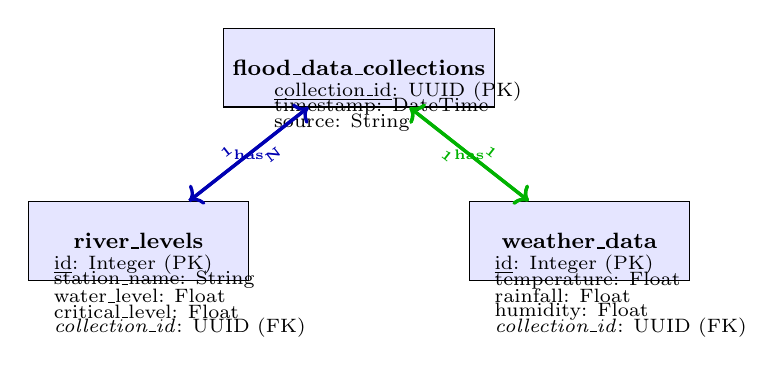
\begin{tikzpicture}[
    entity/.style={draw,rectangle,fill=blue!10,minimum width=2.8cm,minimum height=1.0cm,align=center,font=\footnotesize},
    attr/.style={font=\scriptsize,anchor=west}
  ]
    % Entity: flood_data_collections
    \node[entity] (c) at (0,3.0) {\textbf{flood\_data\_collections}};
    \node[attr] at (-1.2,2.7) {\underline{collection\_id}: UUID (PK)};
    \node[attr] at (-1.2,2.5) {timestamp: DateTime};
    \node[attr] at (-1.2,2.3) {source: String};
    
    % Entity: river_levels
    \node[entity] (r) at (-2.8,0.8) {\textbf{river\_levels}};
    \node[attr] at (-4.0,0.5) {\underline{id}: Integer (PK)};
    \node[attr] at (-4.0,0.3) {station\_name: String};
    \node[attr] at (-4.0,0.1) {water\_level: Float};
    \node[attr] at (-4.0,-0.1) {critical\_level: Float};
    \node[attr] at (-4.0,-0.3) {\textit{collection\_id}: UUID (FK)};
    
    % Entity: weather_data
    \node[entity] (w) at (2.8,0.8) {\textbf{weather\_data}};
    \node[attr] at (1.6,0.5) {\underline{id}: Integer (PK)};
    \node[attr] at (1.6,0.3) {temperature: Float};
    \node[attr] at (1.6,0.1) {rainfall: Float};
    \node[attr] at (1.6,-0.1) {humidity: Float};
    \node[attr] at (1.6,-0.3) {\textit{collection\_id}: UUID (FK)};
    
    % Relationships with cardinality
    \draw[->,very thick,blue!70!black] (c) -- node[above left,font=\tiny,sloped] {\textbf{1}} (r);
    \draw[->,very thick,blue!70!black] (r) -- node[below right,font=\tiny,sloped] {\textbf{N}} (c);
    \node[anchor=center,font=\tiny\bfseries,text=blue!70!black] at (-1.4,1.9) {has};
    
    \draw[<->,very thick,green!70!black] (c) -- node[above right,font=\tiny,sloped] {\textbf{1}} (w);
    \draw[<->,very thick,green!70!black] (w) -- node[below left,font=\tiny,sloped] {\textbf{1}} (c);
    \node[anchor=center,font=\tiny\bfseries,text=green!70!black] at (1.4,1.9) {has};
  \end{tikzpicture}}
  \end{center}
\end{frame}

\begin{frame}[fragile]{FIPA-ACL Message Queue (Core Snippet)}
\begin{lstlisting}
class MessageQueue:
    def __init__(self):
        self.queues: Dict[str, Queue] = {}
        self.lock = Lock()
    def send_message(self, message: ACLMessage) -> bool:
        receiver = message.receiver
        with self.lock:
            if receiver not in self.queues:
                raise ValueError(f"Receiver {receiver} not registered")
            self.queues[receiver].put(message)
            return True
\end{lstlisting}
\end{frame}

\begin{frame}{FloodAgent Data Collection Flow}
  \small
  \begin{enumerate}\itemsep2pt
    \item Scheduled trigger (300s)
    \item PAGASA API (17 stations) \(\rightarrow\) filter to 5
    \item OWM API (weather context)
    \item Combine \& classify
    \item ACL message \(\rightarrow\) MessageQueue
    \item Persist to DB; broadcast via WebSocket
  \end{enumerate}
\end{frame}

\begin{frame}{Haversine Formula Derivation (Sketch)}
  \small
  From spherical law of cosines; numerical stability improved by haversine form. Suitable at city scale.
\end{frame}

\begin{frame}{Dependency Graph Visualization (Sketch)}
  \begin{center}
  \adjustbox{width=0.85\textwidth,center}{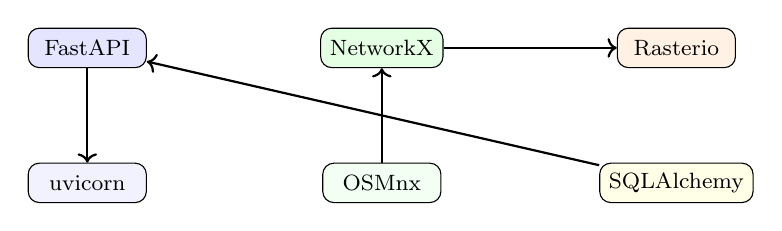
\begin{tikzpicture}[node distance=1.2cm,every node/.style={font=\footnotesize,minimum width=1.5cm,minimum height=0.5cm,align=center}]
    \node[draw,rounded corners,fill=blue!10] (fa) {FastAPI};
    \node[draw,rounded corners,below=of fa,fill=blue!5] (uv) {uvicorn};
    \node[draw,rounded corners,right=2.2cm of fa,fill=green!10] (nx) {NetworkX};
    \node[draw,rounded corners,below=of nx,fill=green!5] (ox) {OSMnx};
    \node[draw,rounded corners,right=2.2cm of nx,fill=orange!10] (rs) {Rasterio};
    \node[draw,rounded corners,below=of rs,fill=yellow!10] (sa) {SQLAlchemy};
    \draw[->,thick] (fa)--(uv);
    \draw[->,thick] (ox)--(nx);
    \draw[->,thick] (nx)--(rs);
    \draw[->,thick] (sa)--(fa);
  \end{tikzpicture}}
  \end{center}
\end{frame}

\begin{frame}{Frontend Component Architecture (Sketch)}
  \small
  \begin{itemize}
    \item \texttt{MapboxMap} (GeoTIFF overlay, route layer, markers)
    \item Hooks: \texttt{useWebSocket}; Context: \texttt{WebSocketContext}
  \end{itemize}
\end{frame}

\begin{frame}{Performance Profiling (If Asked)}
  \small
  \begin{itemize}
    \item A* dominates \(\sim\)60\% CPU
    \item Memory peak \(\sim\)150MB
    \item Opportunities: bidirectional A*, heuristic tuning
  \end{itemize}
\end{frame}

\begin{frame}{Historical Flood Events Dataset (Planned)}
  \small
  \begin{tabular}{lllll}
    \toprule
    Event & Date & Max Level & Impassable Roads & Duration \\
    \midrule
    Ondoy & 2009-09-26 & 21.5m & 50+ & 12h \\
    Ulysses & 2020-11-12 & 18.2m & 30+ & 8h \\
    \bottomrule
  \end{tabular}
\end{frame}

\begin{frame}{Comparative Baseline Design (Planned)}
  \small
  \textbf{MAS-FRO (Current)}: 5 distributed agents; async collection; message-based; robust isolation.\\
  \textbf{Baseline (To Implement)}: Single process; synchronous collection; direct calls; simpler but less robust.
\end{frame}

\end{document}


